\documentclass{beamer}

\usepackage[utf8]{inputenc}
\usepackage[english]{babel}
% \usepackage{palatino}
% \usepackage{graphicx}
% \graphicspath{{./images/}}
% \usepackage{colortbl}
% \usepackage{xcolor}
\usepackage{tikz}
\usepackage{booktabs}
% \usetikzlibrary{shapes,arrows}
% \usetikzlibrary{mindmap,trees}
% \usetikzlibrary{calc}
% \usepackage{pgfplots}
% \pgfplotsset{compat=newest}
% \pgfplotsset{plot coordinates/math parser=false}
% \newlength\figureheight
% \newlength\figurewidth
% \usepackage{ifthen}
\usepackage{subcaption}
% \usepackage{amsthm}
% \usepackage{amsfonts}
% \usepackage{amssymb}
% \usepackage{amsmath}
% \usepackage{eurosym}
% \usepackage{wasysym}

% \addbibresource{../report/Referencias/referencias.bib}

\mode<presentation>{
    % \usetheme{Warsaw}
    \usetheme{Madrid}
    % \usetheme{Frankfurt}
    \usecolortheme{seahorse}
}

\addtobeamertemplate{frametitle}{}{
\vskip-1em
\begin{tikzpicture}[remember picture,overlay]
\node[anchor=north east,yshift=4pt] at (current page.north east) {
\includegraphics[height=0.8cm]{img/ITA_logo.png}};
\end{tikzpicture}}

\title[Orbital Maneuver Optimization]{Optimal Impulsive Orbital Maneuver Synthesis Through Direct Optimization
}

\author[P. K. Puglia]{\small Pedro Kuntz Puglia\inst{1} \and Willer Santos\inst{2} \and Emilien Flayac\inst{3}}

\institute[ITA/AESP]
{
\vspace{0.5cm}
\begin{minipage}{0.5\linewidth}
  \begin{center}
    \inst{1} ITA, Student\\
    \inst{2} ITA, Professor (AESP)\\
    \inst{3} ISAE-SUPAERO, Professor (DISC)
    \vspace{1em}
    
\includegraphics[height=2.5cm]{img/ITA_logo.png}
  \end{center}
\end{minipage}
}

%???
\setbeamertemplate{navigation symbols}{}

\date{}

\begin{document}

\begin{frame}
    \titlepage
\end{frame}

% Recall the outline at each section
\AtBeginSection[]
{%
\begin{frame}
  \frametitle{Plan}
  \small
  %\tableofcontents[hideothersubsections]
  %\tableofcontents[currentsubsection,hideothersubsections]
  \tableofcontents[currentsubsection]
  \normalsize
\end{frame}
}

\section{Introduction}

\begin{frame}{Context}
    \only<1>{
        \begin{figure}[htbp]
            \centering
            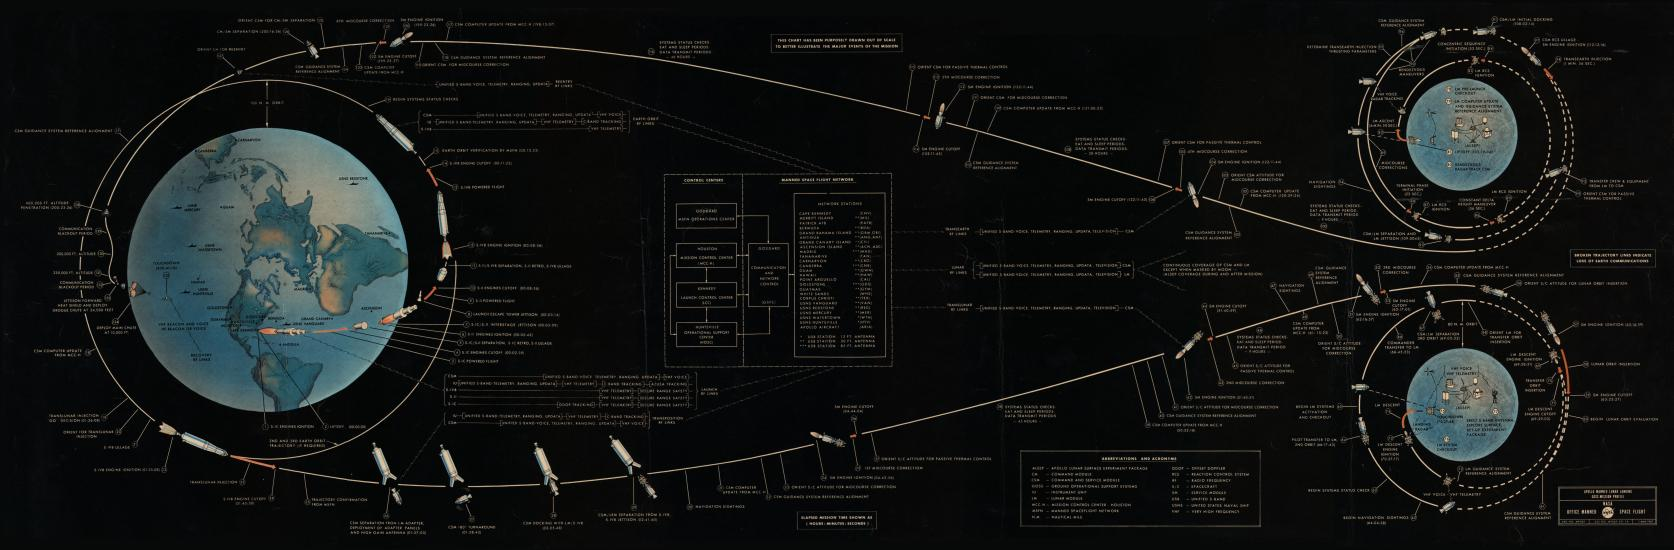
\includegraphics[width=\textwidth]{img/apollo_trajectory.jpg}
            \caption{~\cite{apollo_trajectory}}
            % \label{<label>}
        \end{figure}
    }

    \only<2-3>{
        \begin{figure}
            \centering
            \visible<2-3>{
                \begin{subfigure}{0.4\textwidth}
                    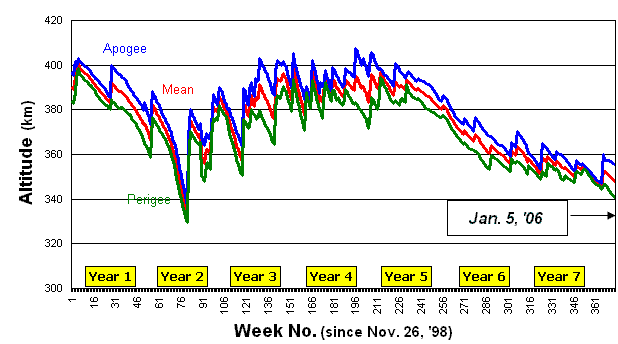
\includegraphics[width=\textwidth]{img/ISS_altitude.png}
                    \caption{~\cite{iss_altitude}}
                \end{subfigure}
            }
            \visible<3>{
                \begin{subfigure}{0.4\textwidth}
                    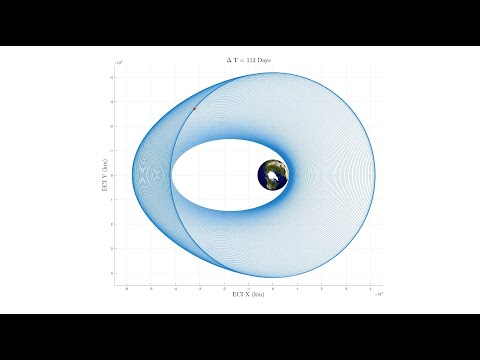
\includegraphics[width=\textwidth]{img/gto_to_geo.jpeg}
                    \caption{~\cite{low_thrust}}
                \end{subfigure}
            }
        \end{figure}
    }

    \only<4-5>{
        \begin{figure}
            \centering
            \visible<4-5>{
                \begin{subfigure}{0.4\textwidth}
                    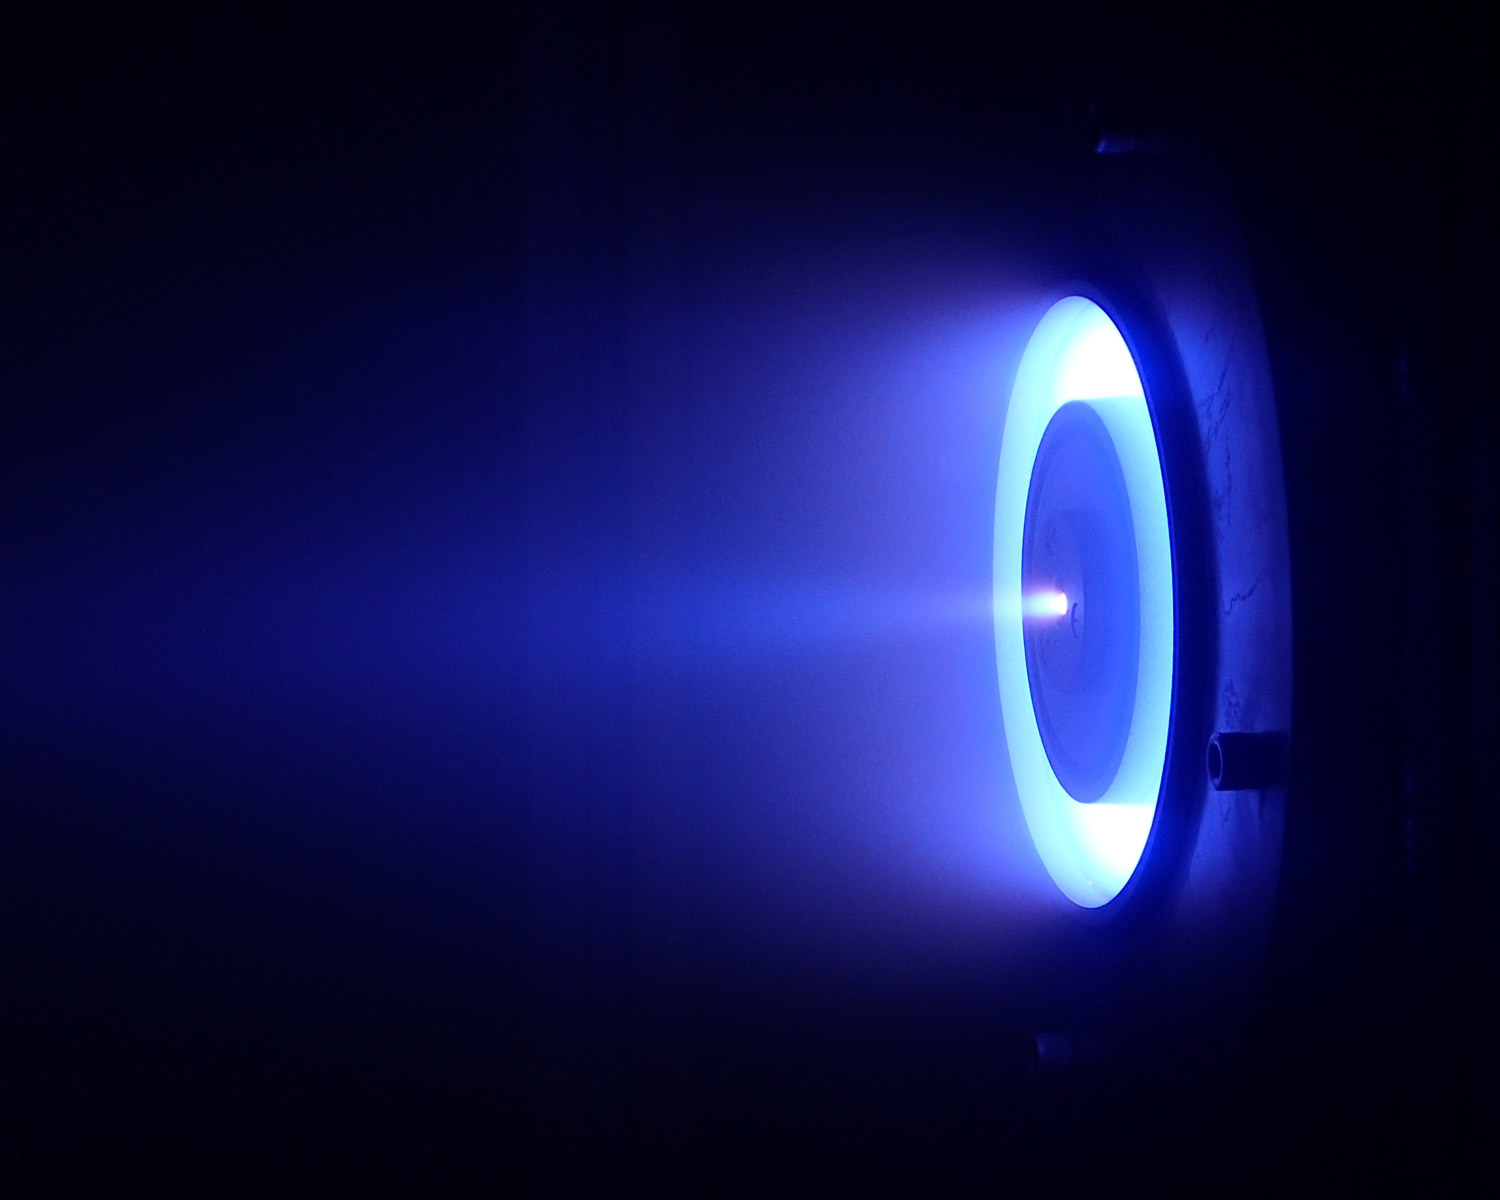
\includegraphics[width=\textwidth]{img/hall_effect.jpg}
                    \caption{~\cite{hall_effect}}
                \end{subfigure}
            }
            \visible<5>{
                \begin{subfigure}{0.4\textwidth}
                    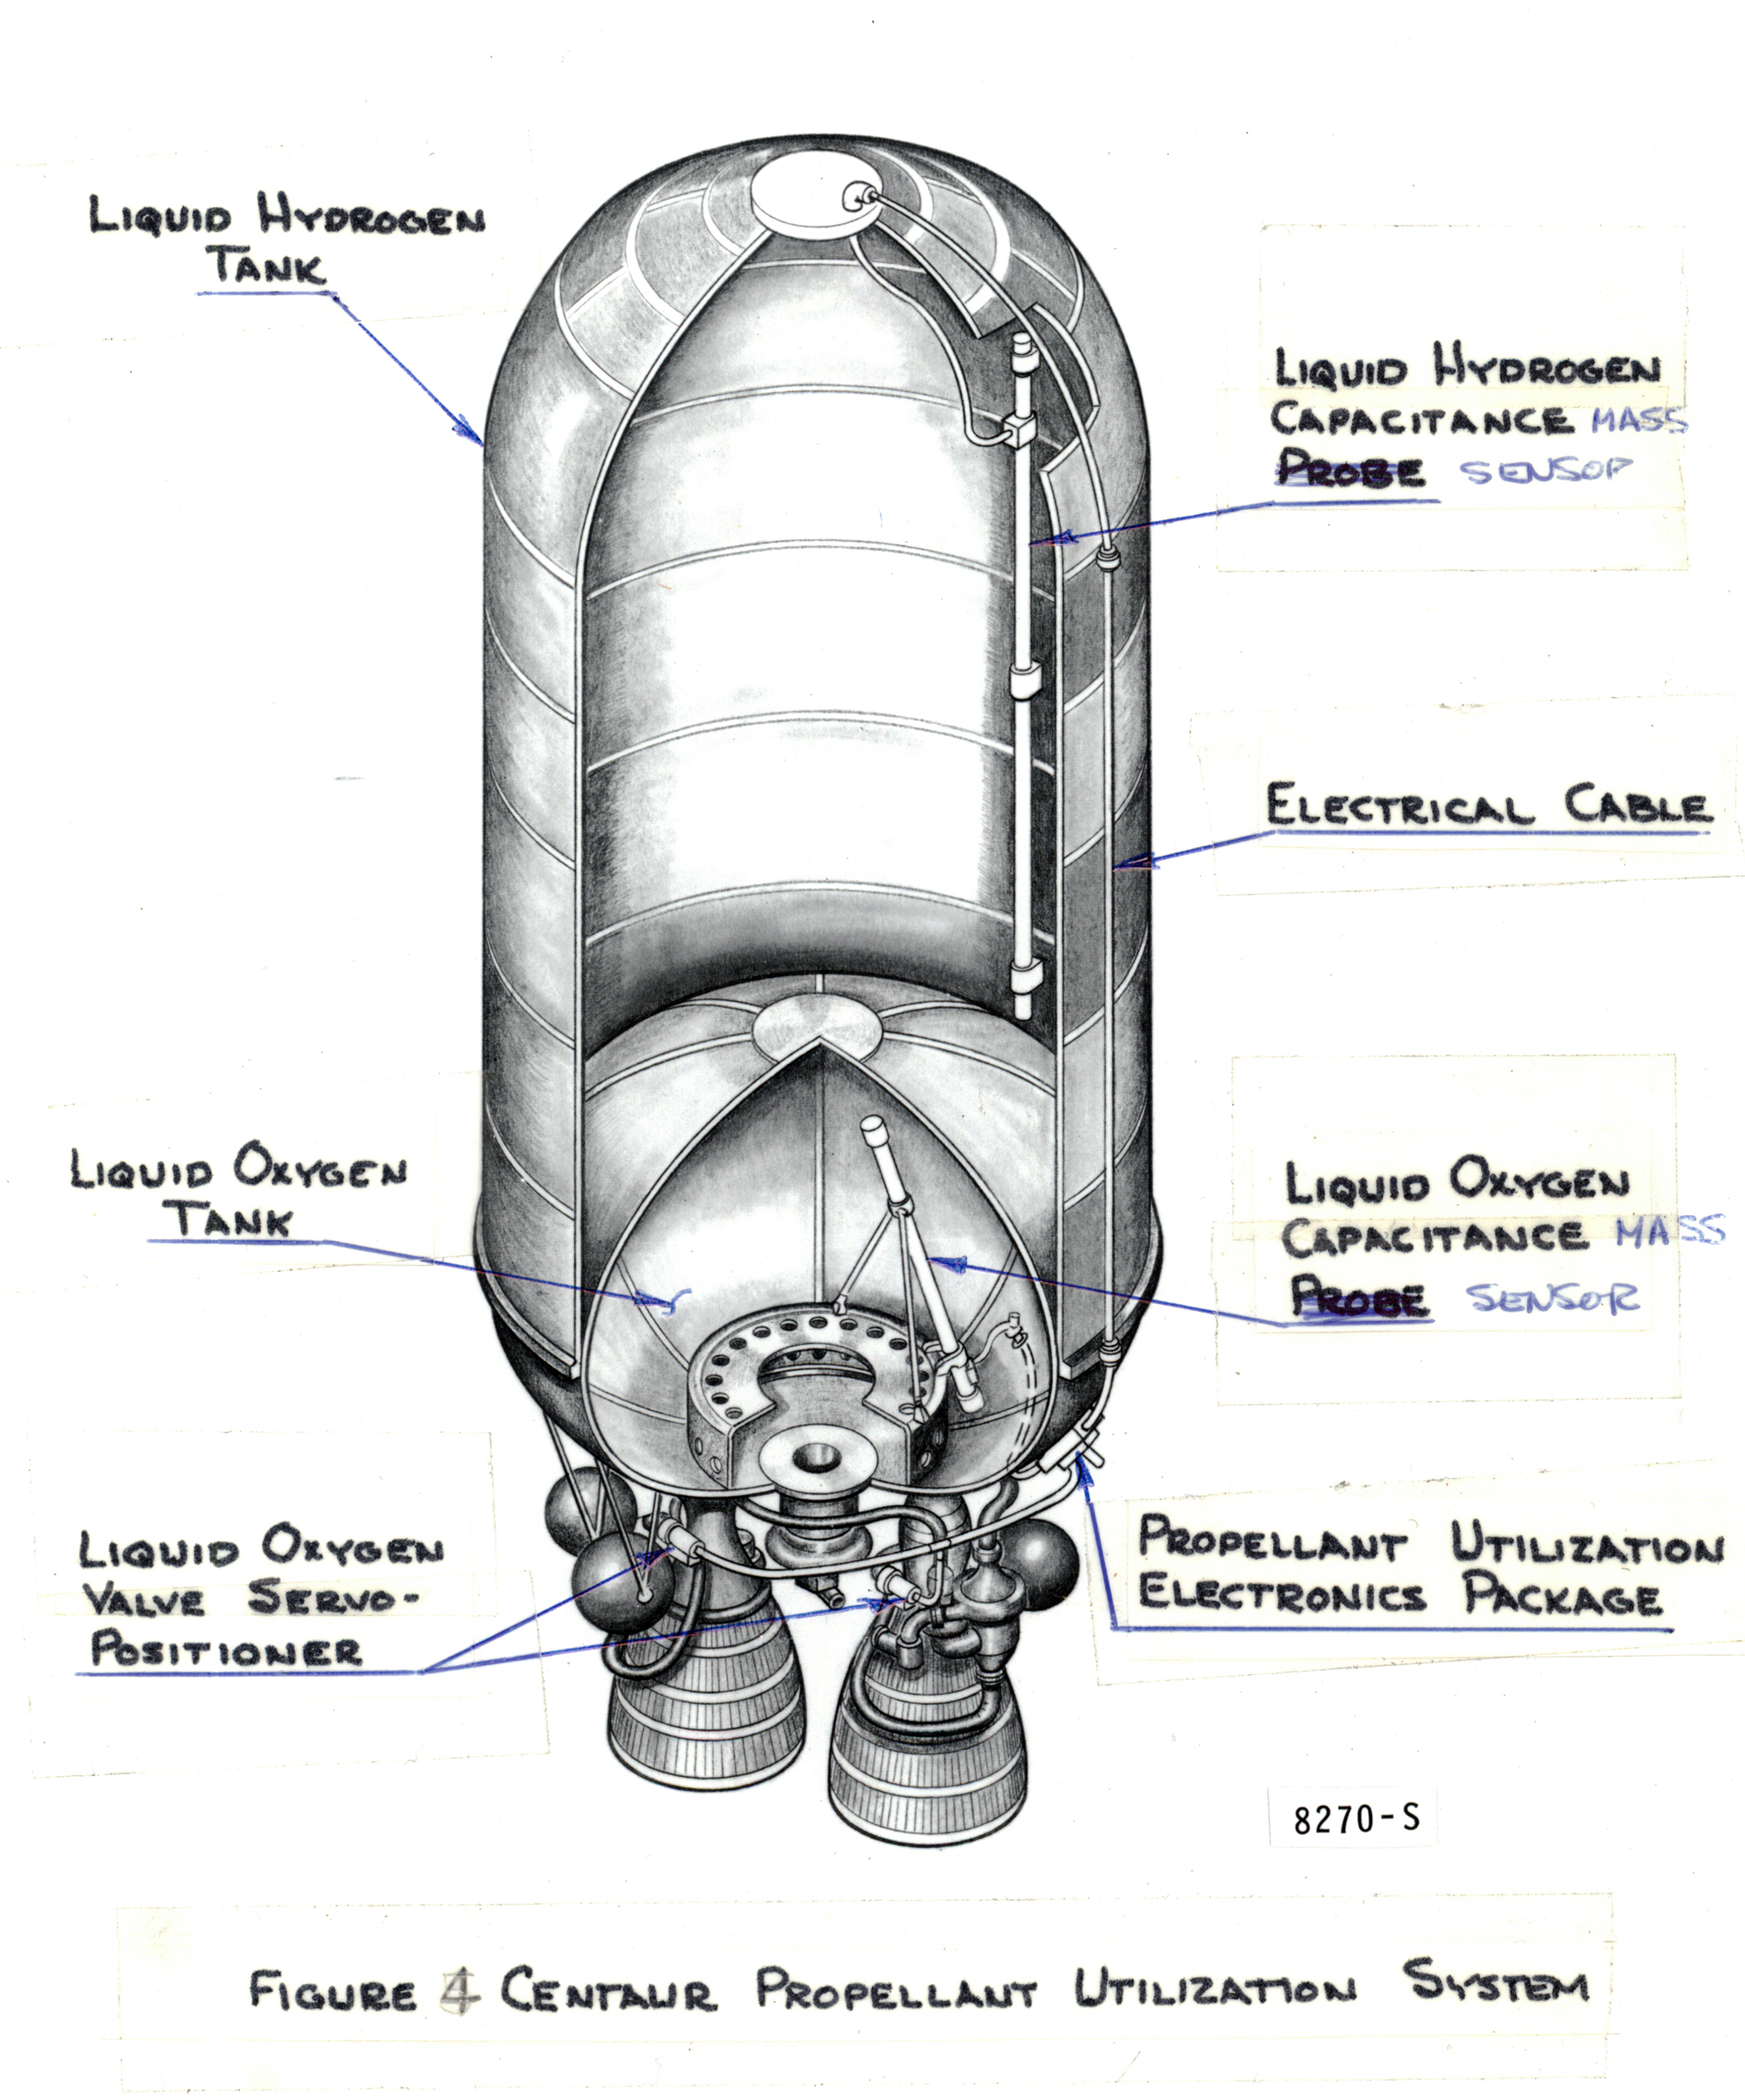
\includegraphics[width=\textwidth]{img/Centaur-propellant-system.jpg}
                    \caption{~\cite{centaur}}
                \end{subfigure}
            }
        \end{figure}
    }
\end{frame}

\begin{frame}{Problem Statement}
    \begin{block}{Central Question}
        What is the most efficient sequence of maneuvers that takes a spacecraft from an initial state to a final state in a given time?
    \end{block}
    
    \begin{itemize}
        \item Efficient: least propellant usage
        \item General case in mind (no particular analytical solutions)
        \item How much time? Feasibility, trade-offs?
        \item How many impulses?
        \item Is it optimal?
    \end{itemize}
\end{frame}

\begin{frame}
    \frametitle{Hypotheses}

    \begin{itemize}
        \item Choice for \textit{impulsive propulsion} \(\rightarrow\) reducible to parameter optimization
        \item Good numerical solvers: Ipopt\cite{ipopt}
        \item Many local optima (non-convex problem)
        \item Expect \textit{Primer vector} theory provides (some) solutions
    \end{itemize}
\end{frame}

\begin{frame}
    \frametitle{Objectives}

    \begin{itemize}
        \item Apply primer vector theory;
        \item Study how much time fo transfer, and how to find it;
        \item Compare numerical and analytical results;
        \item Discuss applications in common scenarios;
    \end{itemize}

\end{frame}

\begin{frame}
    \frametitle{Justification}

    Some institutions already know how to optimize orbital maneuvers. Why study it again?

    \begin{figure}[htbp]
        \centering
        \begin{subfigure}{0.25\textwidth}
            
\includegraphics[width=\textwidth]{img/orekit-logo.png}
            \caption{Orekit library provides maneuver analysis, and indirect optimization (outdated).}
        \end{subfigure}
        \begin{subfigure}{0.25\textwidth}
            
\includegraphics[width=\textwidth]{img/patrius_logo.png}
            \caption{CNES Patrius library provides analysis, not Synthesis.}
        \end{subfigure}
        \begin{subfigure}{0.25\textwidth}
            \centering
            
\includegraphics[width=\textwidth]{img/mystic_no_download.png}
            \caption{NASA's Mystic software (Dawn Discovery mission) is not available for download.}
        \end{subfigure}
    \end{figure}

    \textbf{No widely available orbital maneuver optimization software.}
\end{frame}

\section{Theory}

\begin{frame}
    \frametitle{Theory components}

    \begin{figure}[htbp]
        \centering
        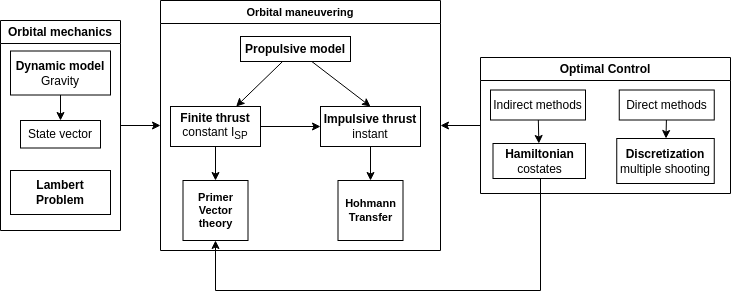
\includegraphics[width=\textwidth]{img/theory_components.png}
        % \caption{<caption>}
        % \label{<label>}
    \end{figure}
\end{frame}

\begin{frame}
    \frametitle{Orbital mechanics}

    \begin{block}{Two-Body Motion}
        Keplerian dynamics:
        \begin{equation}
            \ddot{\mathbf{r}} = - \frac{\mu}{\lVert \mathbf{r} \rVert^3} \mathbf{r}
        \end{equation}
        Closed, periodic elliptical trajectory for negative energy (bound satellite).
    \end{block}
    \begin{columns}
        \begin{column}{0.5\linewidth}
            State vector choice:
            \begin{itemize}
                \item \textbf{Cartesian}: \(\mathbf{x} = \begin{bmatrix}
                    \mathbf{r}\ \textit{(position)} \\ \mathbf{v}\ \textit{(velocity)} 
                \end{bmatrix}\)
                \item \textbf{Keplerian} (elliptical orbit only): \(\mathbf{x} = \begin{bmatrix}
                    a\ \textit{(semi-major axis)}\\ 
                    e\ \textit{(eccentricity)} \\ 
                    i\ \textit{(inclination)} \\ \Omega\ \textit{(RAAN)} \\ \omega\ \textit{(argument of perigee)} \\ \theta\ \textit{(true anomaly)}
                \end{bmatrix}\)
            \end{itemize}
        \end{column}
        \begin{column}{0.5\linewidth}
            COLOCAR FIGURA
        \end{column}
    \end{columns}
\end{frame}

\begin{frame}
    \frametitle{Lambert Problem}
    \begin{block}{Statement}
        What is the orbit of a satellite that passes by position \(\mathbf{r}_2\) at a time \(\Delta t\) after being in position \(\mathbf{r}_1\)?
    \end{block}
    \begin{itemize}
        \item \textbf{Importance}: auxiliary role in orbital maneuvering (feasible transfer);
        \item If \(\mathbf{v_1}\) is found, problem is solved;
        \item Issue with \(\mathbf{r}_1 \parallel \mathbf{r}_2\) (eg, perigee \& apogee): orbit plane unknown
        \item Universal variable formulations: simple, cannot handle indetermination~\cite{curtis2015orbital}\cite{sukhanov}
        \item Cartesian formulation~\cite{embedded_lambert}
    \end{itemize}
\end{frame}

\begin{frame}
    \frametitle{Optimal control}
    \begin{block}{Generic optimal control problem}
        Given a dynamical system \(\dot{\mathbf{x}} = f(\mathbf{x}, \mathbf{u})\), a fixed initial condition \(\mathbf{x}(0) = \mathbf{x}_i\), a total time \(t_f\) and a final condition \(\mathbf{x}(t_f) = \mathbf{x}_f\), find control trajectory \(\mathbf{u}(t)\) minimizing (max.) objective \(J[\mathbf{x}(t), \mathbf{u}(t)] = h(\mathbf{x}(t_f))+\int_0^{t_f} L(x(t), u(t)) dt\).
        % \(\mathbf{u}(t)\) 
    \end{block}
    \begin{columns}
        \begin{column}{0.5\linewidth}
            \begin{center}
                \textbf{Indirect method}
            \end{center}
            \begin{itemize}
                \item Hamiltonian~\cite{bertsekas}: \(H = L(\mathbf{x}, \mathbf{u}) + \mathbf{\lambda}^T f(\mathbf{x}, \mathbf{u})\)
                \item costate \(\mathbf{\lambda}\)
                \item Pontryagin's Minimum Principle:
                \begin{equation}
                    \mathbf{u} = \arg \min_{\mathbf{u} \in \mathcal{U}} H[\mathbf{x}, \mathbf{u}, \mathbf{\lambda}].
                \end{equation}
                \item Solve for \(\mathbf{x}\), \(\mathbf{\lambda}\), \(\mathbf{u}\)
            \end{itemize}
        \end{column}
        \begin{column}{0.5\linewidth}
            \begin{center}
                \textbf{Direct method}
            \end{center}
            \begin{itemize}
                \item Discretize time, diff.\ eq.
                \item Numerical integration: Euler, RK4, RK8
                \item Trajectories \(\rightarrow \mathbf{x}_k, \mathbf{u}_k\)
                \item Parameter optimization
                \item Solve for \(\mathbf{x}\), \(\mathbf{u}\)
            \end{itemize}
        \end{column}
    \end{columns}
\end{frame}

\begin{frame}
    \frametitle{Orbital Maneuvering}

    \begin{block}{Extended dynamics}
        \begin{equation}
            \ddot{\mathbf{r}} = -\frac{\mu}{\lvert \mathbf{r} \rVert^3}\mathbf{r} + \frac{\mathbf{F}}{m}.
        \end{equation}
        Thrust \(\mathbf{F}\) related to mass \(m\) through \textit{propulsion model}.
    \end{block}

    \begin{columns}
        \begin{column}{0.5\linewidth}
            \begin{center}
                \textbf{Finite Thrust}
            \end{center}
            \begin{itemize}
                \item \(F = - \dot m v_e\)
                \item constant exhaust velocity \(v_e\) and specific impulse \(v_e = I_{sp} g_0\) (CSI)
                \item \(F \leq F_{\max}\)
                \item Extra state: mass
            \end{itemize}
        \end{column}
        \begin{column}{0.5\linewidth}
            \begin{center}
                \textbf{Impulsive thrust} (\(F_{\max} \rightarrow \infty\))
            \end{center}
            \begin{itemize}
                \item Discrete impulses, \textit{coasting arcs}
                \item Tsiolkovsky's Equation~\cite{curtis2015orbital}:
                \begin{equation}
                    \Delta v = v_e \ln{\left(\frac{m_i}{m_f}\right)}
                \end{equation}
                \item \(\mathbf{v}(t_i^+) = \mathbf{v}(t_i^-) + \Delta \mathbf{v} \)
                \item \(\min \int -\dot m \text{dt} \leftrightarrow \min \sum \Delta v_i \)
            \end{itemize}
        \end{column}
    \end{columns}  
\end{frame}

\begin{frame}
    \frametitle{Primer vector theory}

    \begin{columns}
        \begin{column}{0.7\linewidth}
            \begin{itemize}
                \item Apply Hamiltonian to finite thrust CSI case~\cite{Conway_2010} (\(\int \dot m dt \ll m(0)\))
                \item \textit{primer vector} \(\mathbf{p} = - \mathbf{\lambda}_v\) (velocity costate)
                \item Optimal thrust statisfies (\textit{bang-bang})
                \begin{equation}
                    \mathbf{F} = \begin{cases}
                        F_{\max} \frac{\mathbf{p}}{p}&, p > 1 \\
                        0&, p < 1
                    \end{cases}
                \end{equation}
                \item Extension to impulsive case
                \begin{enumerate}
                    \item \(\mathbf{p}(t)\) and \(\dot{\mathbf{p}}(t)\) continuous;
                    \item \(\lVert \mathbf{p} \rVert \leq 1\), impulses happen when \(\lVert \mathbf{p} \rVert = 1\);
                    \item \(\mathbf{p}\) has the direction of impulse at the impulse instants;
                    \item \(\frac{d \lVert \mathbf{p} \rVert}{dt} = 0\) at impulses at \(t \in (0, t_f)\).
                \end{enumerate}
                \item \(p(t)\) analytical in coasting arcs
            \end{itemize}
        \end{column}
        \begin{column}{0.3\linewidth}
            \begin{figure}[htbp]
                \centering
                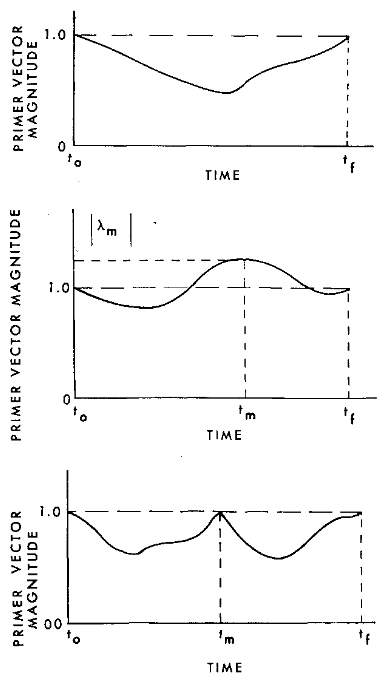
\includegraphics[width=\linewidth]{img/primer_vector_history_from_jezewsky.png}
                % \caption{<caption>}
                % \label{<label>}
            \end{figure}
        \end{column}
    \end{columns}      
\end{frame}

\section{Methodology}

\begin{frame}
    \frametitle{Numerical Tools}

    \begin{itemize}
        \item Julia~\cite{Julia-2017} language
        \item \texttt{SatelliteToolbox}~\cite{satellitetoolbox}: INPE's own orbit propagator
        \item \texttt{JuMP}~\cite{jump}: optimization modelling sub-language
        \item Ipopt~\cite{ipopt}: robust nonlinear optimizer. Local, deterministic, grandient-based
    \end{itemize}
    
    \begin{figure}[htbp]
        \centering
        \begin{subfigure}{0.24\textwidth}
            
\includegraphics[width=\textwidth]{img/julia.png}
        \end{subfigure}
        \begin{subfigure}{0.24\textwidth}
            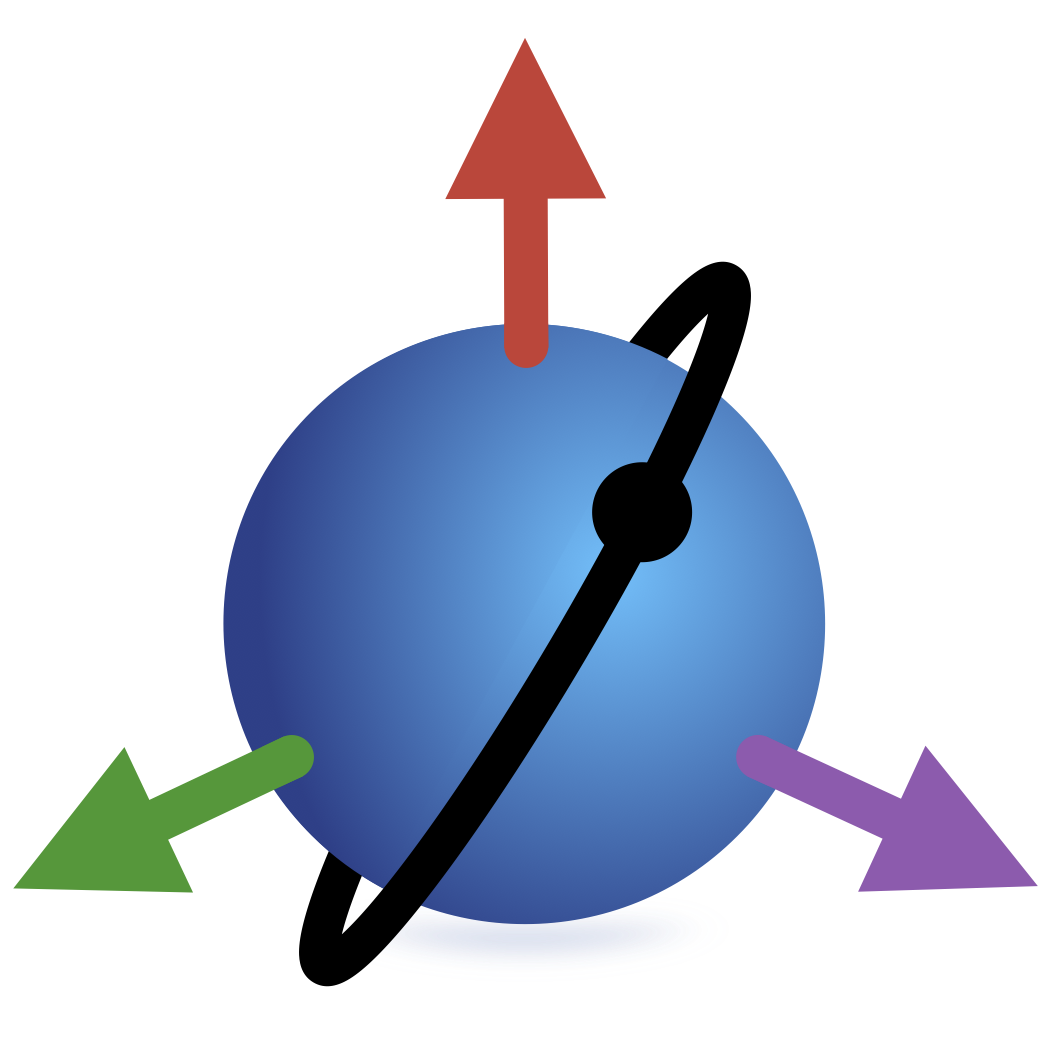
\includegraphics[width=\textwidth]{img/satellitetoolbox_logo.png}
        \end{subfigure}
        \begin{subfigure}{0.24\textwidth}
            
\includegraphics[width=\textwidth]{img/jump_logo.png}
        \end{subfigure}
        \begin{subfigure}{0.24\textwidth}
            
\includegraphics[width=\textwidth]{img/ipopt_logo.png}
        \end{subfigure}
        % \caption{<caption>}
        % \label{<label>}
    \end{figure}
\end{frame}

\begin{frame}
    \frametitle{Modelling}

    \begin{itemize}
        \item Coasting arc model
        \begin{itemize}
            \item Dynamics discretized with RK4 \(\mathbf{x}_{\text{next}} = f_{RK}(\mathbf{x}_{\text{prev}}, \Delta t)\), \(N\) steps
            \item \(N+1\) state vectors \(\mathbf{x}^j\) related by
            \begin{equation}
                 \mathbf{x}^{j+1} = f_{RK}(\mathbf{x}^j, \frac{t_p}{N}), j = 1, \dots, N
            \end{equation}
            \item 6 DoF left
            \item \(\mathbf{x}^1\) given: propagation
            \item \(\mathbf{r}^1\), \(\mathbf{r}^{N+1}\) given: Cartesian Lambert solver
        \end{itemize}
        \item Two impulse model
        \begin{itemize}
            \item 3 coasts \(\mathbf{x}^j_c\), \(j=1,\dots,N+1\), \(c=1,2,3\)
            \item \(\Delta v_i\), \(\hat{\mathbf{u}}_i\), \(i = 1, 2\) such that \(\lVert \hat{\mathbf{u}}_i \rVert = 1\) and \(\mathbf{x}_{i+1}^1 = \mathbf{x}_i^{N+1} + \begin{bmatrix}
                0_{3\times1} \\ \Delta v_i \hat{\mathbf{u}}_i
            \end{bmatrix}, m=1, 2\)
            \item variable impulse intervals s.t. \(\Delta t_1 + \Delta t_2 \leq t_f\)
        \end{itemize}
    \end{itemize}
\end{frame}

\section{Results}

\begin{frame}
    \frametitle{Expected Results}

    \begin{itemize}
        \item More robust code
        \begin{itemize}
            \item perturbed orbital dynamics (easy)
            \item multiple impulses (medium);
            \item better convergence guarantees (unknown);
            \item multiple revolution transfers (hard)
        \end{itemize}
        \item Estimation of transfer time \(t_f\) instead of arbitrary input~\cite{embedded_lambert}
        \item Practical orbital transfer cases under appropriate models:
        \begin{enumerate}
            \item LEO maintenance: inclination and altitude;
            \item SSO maintenance: inclination, RAAN and semimajor-axis;
            \item Constellation phasing: change phase along orbit
            \item LEO to GEO transfer: multiple impulse, small plane change, numerical challenge (different time and spatial scales between the start and the end)
        \end{enumerate}
    \end{itemize}

\end{frame}

\begin{frame}
    \frametitle{Preliminary Results}

    \begin{block}{Goal}
        Reproduce Hohmann transfer numerically.
        
    \end{block}

    \begin{table}[htbp]
        \centering
        \begin{tabular}{ccc} \toprule
            Element & Initial & Final \\ \midrule
            \(a\)      & \(7000\) km   & \(9000\) km   \\
            \(e\)      & \(0\)        & \(0\)        \\
            \(i\)      & \(51^\circ\) & \(51^\circ\) \\
            \(\Omega\) & \(0^\circ\)  & \(0^\circ\)  \\
            \(\omega\) & \(0^\circ\)  & \(0^\circ\)  \\
            \(\theta\) & \(0^\circ\)  & \(180^\circ\)  \\ \bottomrule
        \end{tabular}
        \caption{Orbital elements used for the Hohmann transfer case analysis}
        \label{tab:hohmann_orb_elems}
    \end{table}

    
\end{frame}

\begin{frame}
    \frametitle{Analytical Solution}
    
    
    \begin{figure}[htbp]
        \centering
        \begin{subfigure}{0.49\textwidth}
            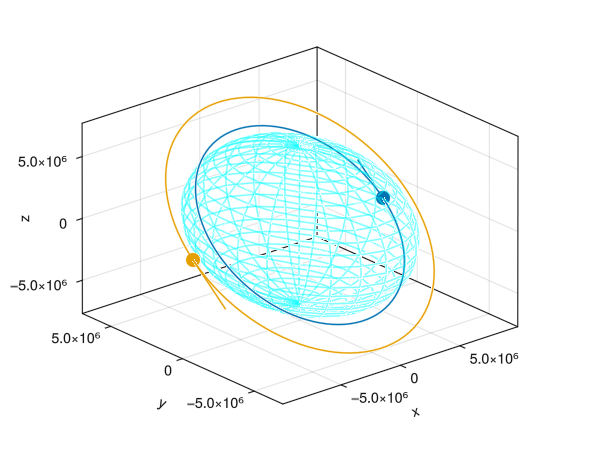
\includegraphics[width=\textwidth]{../report/img/hohmann_condition.png}
            \caption{3D view.}
        \end{subfigure}
        \begin{subfigure}{0.49\textwidth}
            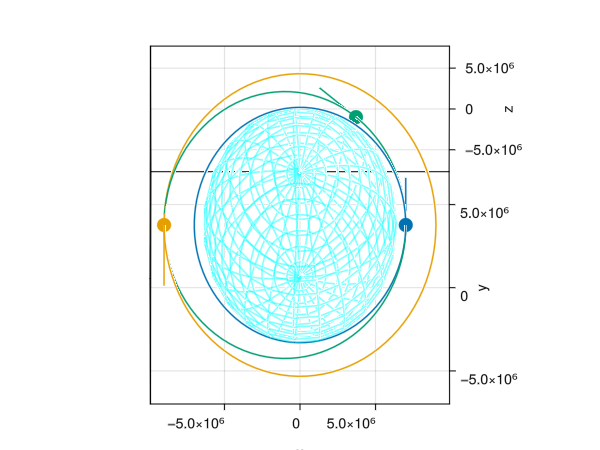
\includegraphics[width=\textwidth]{../report/img/hohmann_condition_in_plane.png}
            \caption{Orbital plane view.}
        \end{subfigure}
        % \caption{Initial (blue), tranfer (green) and final (yellow) orbits for Hohmann transfer case visualization.}
        \label{fig:hohmann_condition}
    \end{figure}
    \textbf{Variables}: \(t_f = 3560.54\) s, \(\sum \lVert \Delta \mathbf{v} \rVert = 887.56\) m/s
\end{frame}

\begin{frame}
    \frametitle{Lambert Problem solution}
    \begin{itemize}
        \item \(t_f\) set to analytical time (cheating!)
        \item Initial guesses \(\Delta t_1\) and \(\Delta t_2\): \(\frac{t_f}{3}\)
        \item Coast, impulse, Lambert solution, impulse, coast: feasible but non-optimal
    \end{itemize}
    
    \begin{figure}[htbp]
        \centering
        \begin{subfigure}{0.49\textwidth}
            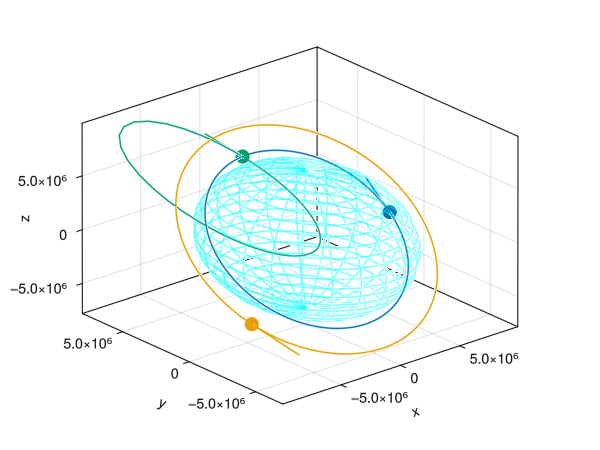
\includegraphics[width=\textwidth]{../report/img/hohmann_lambert_guess.png}
            \caption{3D view.}
        \end{subfigure}
        \begin{subfigure}{0.49\textwidth}
            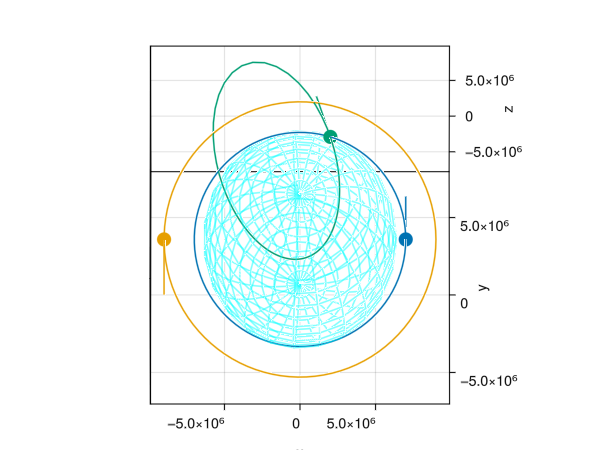
\includegraphics[width=\textwidth]{../report/img/hohmann_lambert_guess_in_plane.png}
            \caption{Orbital plane view.}
        \end{subfigure}
        % \caption{Lambert problem solution for second coasting arc in Hohmann transfer case. This solution will serve as initial guess for the optimizer.}
        \label{fig:hohmann_lambert}
    \end{figure}

\end{frame}

\begin{frame}
    \frametitle{Optimized solution}
    \begin{columns}
        \begin{column}{0.3\textwidth}\centering
            \(N = 50\)
        \end{column}
        \begin{column}{0.7\textwidth}
            \begin{table}[htbp]
                \centering
                \begin{tabular}{ccc} \toprule
                    Variable & Analytical & Solver \\ \midrule
                    \(\Delta t_1\) & 0s & 8e-4s \\
                    \(\Delta t_2\) & 3560.54s & 3560.538s \\
                    \(\sum \lVert \Delta \mathbf{v} \rVert\) & \(887.56m/s\) & \(887.56m/s\) \\ \bottomrule
                \end{tabular}
                % \caption{Comparison of optimized and analytical values of some important variables in the Hohmann transfer case.}
                \label{tab:hohmann_results}
            \end{table}
        \end{column}
    \end{columns}
    
    \begin{figure}[htbp]
        \centering
        \begin{subfigure}{0.49\textwidth}
            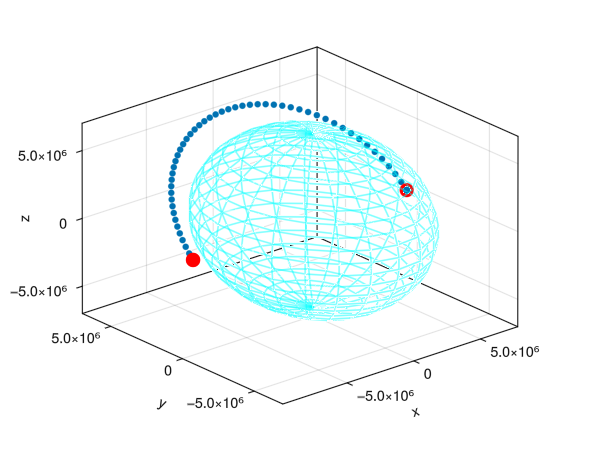
\includegraphics[width=\textwidth]{../report/img/hohmann_solved.png}
            \caption{3D view.}
        \end{subfigure}
        \begin{subfigure}{0.49\textwidth}
            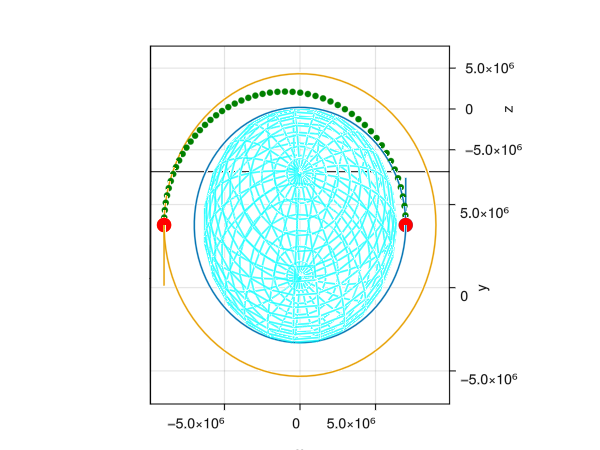
\includegraphics[width=\textwidth]{../report/img/hohmann_solved_in_plane.png}
            \caption{Orbital plane view.}
        \end{subfigure}
        % \caption{Discretized transfer trajectory found by the numerical solver for the Hohmann transfer case.}
        \label{fig:hohmann_traj}
    \end{figure}
    

\end{frame}

\begin{frame}[allowframebreaks]{References}
    \bibliographystyle{plain}
    \bibliography{Referencias/referencias}
\end{frame}

\end{document}